\chapter{Optymalizacja wydajności aplikacji} % (fold)
\label{cha:rekonfigurowalnosc}

\paragraph{} % (fold)
\label{par:}
W celu poprawienia wydajności aplikacji oraz sprawdzenia zachowania w przypadku obciążenia dużą liczbą jednoczesnych zapytań pobierających rekordy z bazy danych, przeprowadzone zostały testy obciążeniowe. Jako środowisko testowe, wykorzystany został program \textit{Gatling Tool \footnote{Gatling Tool - http://gatling-tool.org/}}. Gatling Tool jest wolnym oprogramowaniem cechującym się:
\begin{itemize}
 	\item wysoką wydajnością,
 	\item prostotą założeń,
 	\item wsparciem dla protokołu \textit{HTTP},
 	\item możliwością nagrywania scenariuszy,
 	\item złożoną analizą rezultatów.
 \end{itemize} 

\paragraph{} % (fold)
\label{par:}
Gatling Tool jest programem napisanym w języku \textit{Scala \footnote{Scala - http://scala.org}} i działającym na wirtualnej maszynie javy. Dzięki temu, teoretycznie, testy można przeprowadzić w każdym systemie wspierającym technologie \textit{JVM}. Komputer testowy miał następujące parametry:
\begin{itemize}
	\item procesor: Intel Pentium i5 - 2,3 GHz,
	\item pamięć RAM: 8GB DDR3,
	\item sytem operacyjny: OSX 10.8 Mountain Lion.
\end{itemize}

\paragraph{} % (fold)
 \label{par:}
 Aplikacja internetowa została wdrożona na serwerze o następujących parametrach:
 \begin{itemize}
 	\item procesor: Intel Pentium Dual Core 1,83 GHz,
 	\item pamięć RAM: 3 GB DDR2,
 	\item system operacyjny: Windows 7,
 	\item oprogramowanie: IIS 7, Microsoft SQL Server 2012.
 \end{itemize}


 \paragraph{} % (fold)
 \label{par:}
 Scenariusz testów obejmował załadowanie strony głównej aplikacji, a następnie wyświetlenie profilu o id=1 i id=2. Testy wykonane zostały dla zmiennej liczby użytkowników od 1 do 10000 (1, 10, 100, 1000, 2000, ..., 10000). Wyniki symulacji przedstawione zostały na Rysunkch \ref{fig:sred1} i \ref{fig:got1}
 % paragraph  (end)

\begin{figure}[ht]
	\centering
		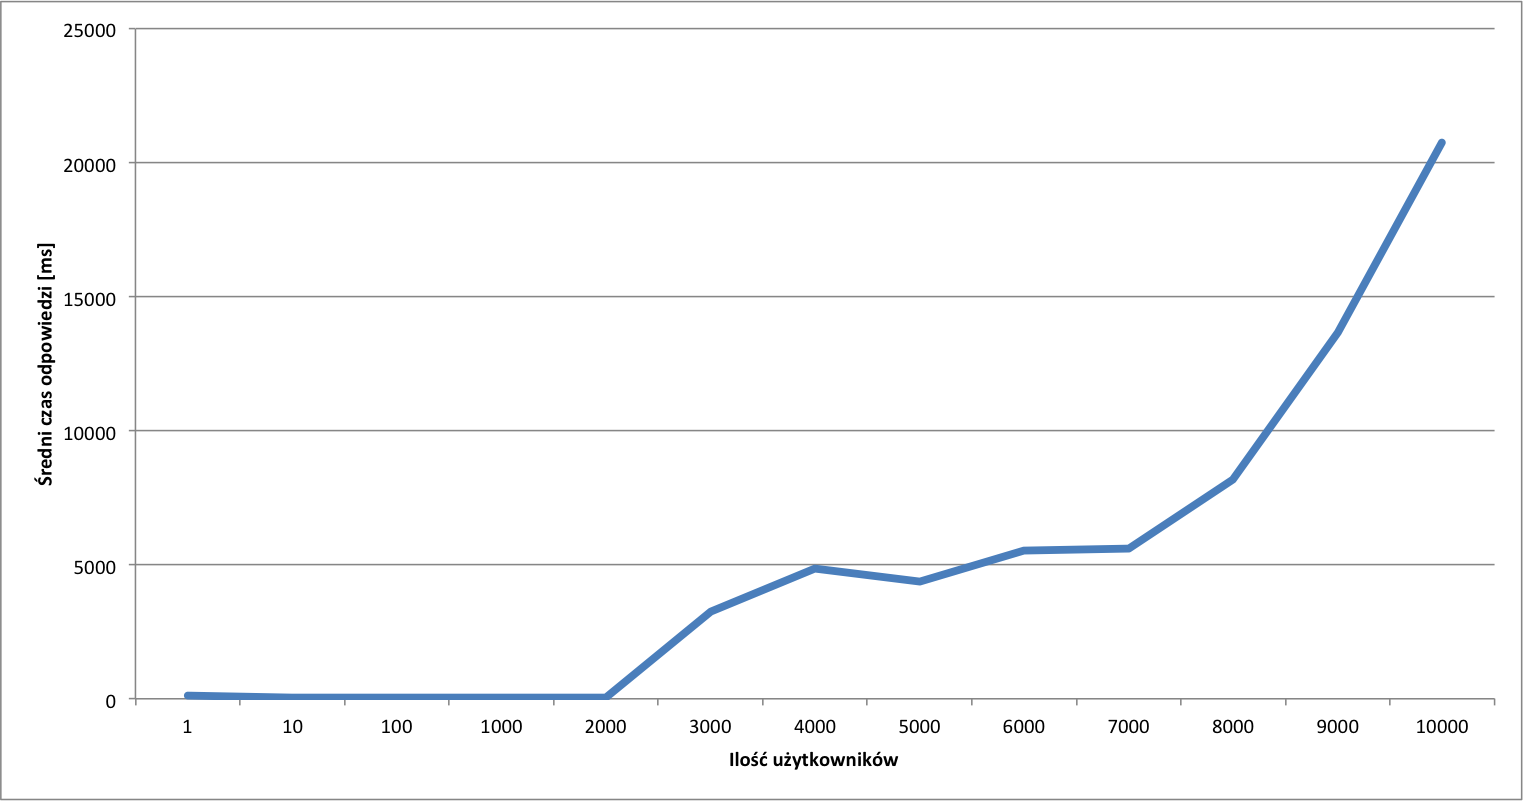
\includegraphics[width=1\linewidth]{assets/sredni1.png}
		\caption{Przebieg średniego czasu odpowiedzi dla całego testu}
	\label{fig:sred1}
\end{figure}

\begin{figure}[ht]
	\centering
		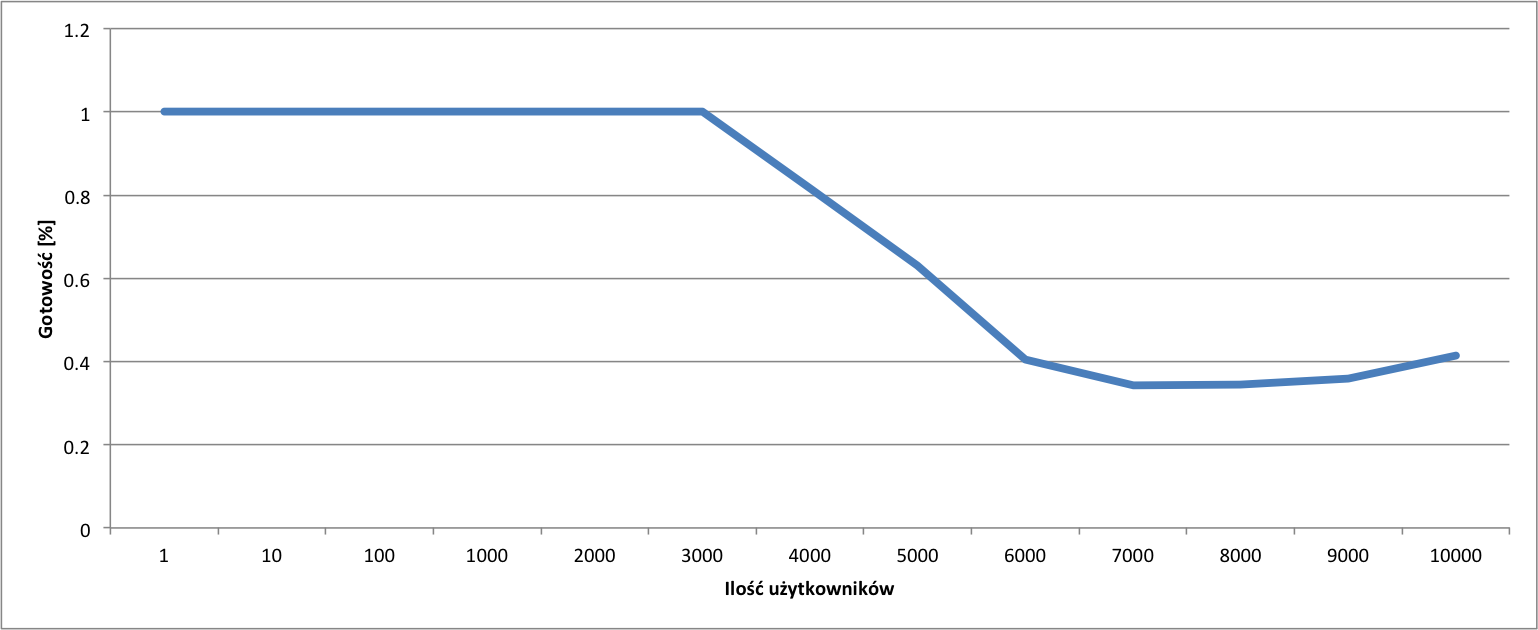
\includegraphics[width=1\linewidth]{assets/gotowosc1.png}
		\caption{Przebieg gotowości systemu dla całego testu}
	\label{fig:got1}
\end{figure}

\paragraph{} % (fold)
\label{par:}
Z danych odczytanych na wykresach (Rysunek \ref{fig:sred1} i \ref{fig:got1}) można zauważyć, że istotny z punktu poprawy wydajności systemu jest zakres jednoczesnych użytkowników systemu od 2000 - 5000. Powyżej 7000 użytkowników, komputer testowy nie nadążał obsługiwać wszytskich przychodzących rządań, powodując błędy programu testowego. Na Rysunkach \ref{fig:sred2} i \ref{fig:got2} przedstawiono wyniki dokładniejszego próbkowania zakresu użytkowników 2000 - 5000.

\begin{figure}[ht]
	\centering
		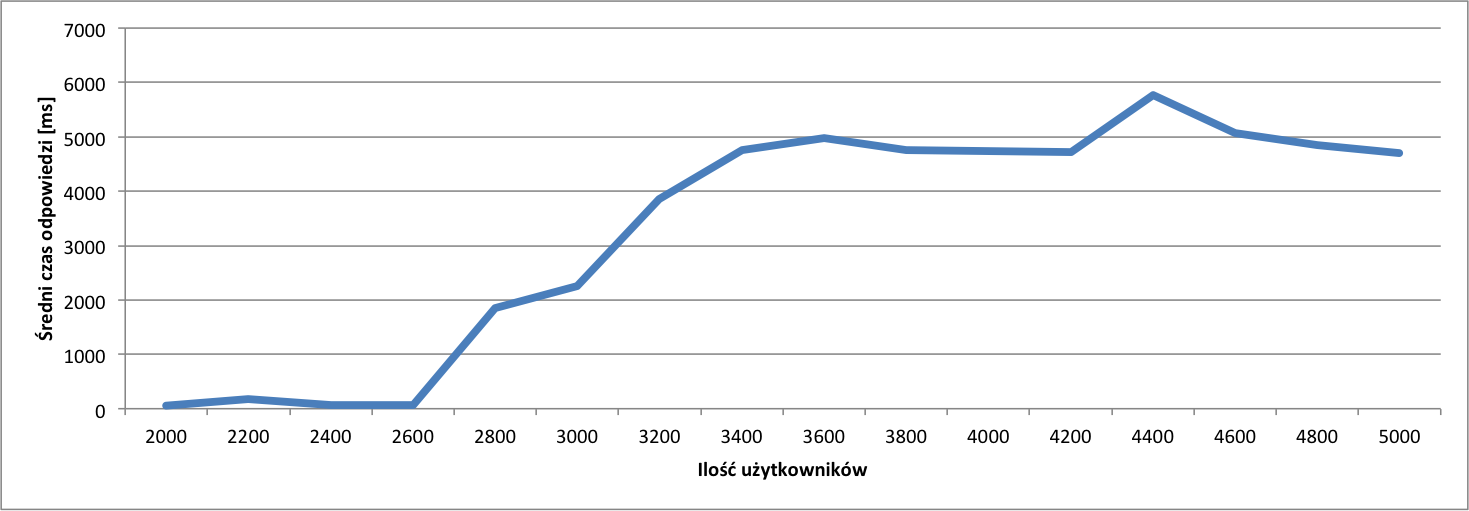
\includegraphics[width=1\linewidth]{assets/sredni2.png}
		\caption{Przebieg średniego czasu odpowiedzi dla zakresu użytkowników od 2000 do 5000}
	\label{fig:sred2}
\end{figure}

\begin{figure}[ht]
	\centering
		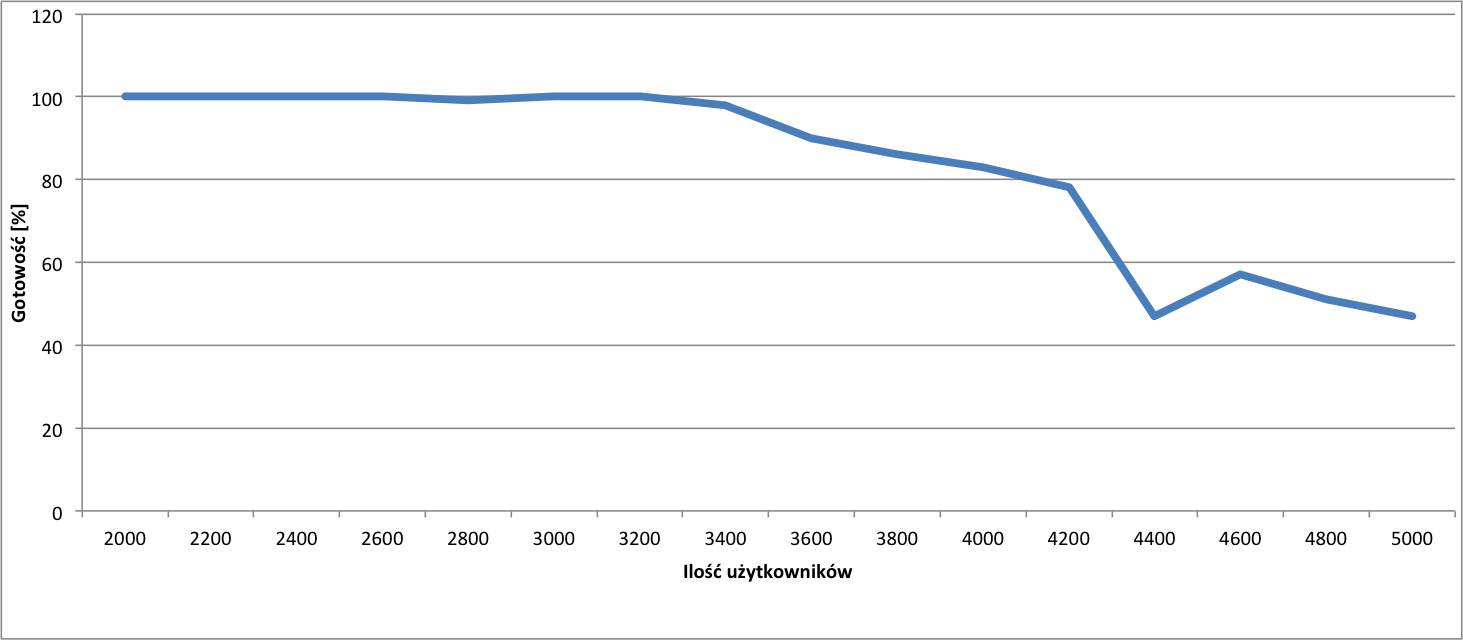
\includegraphics[width=1\linewidth]{assets/gotowosc2.png}
		\caption{Przebieg gotowości systemu dla zakresu użytkowników od 2000 do 5000}
	\label{fig:got2}
\end{figure}
% paragraph  (end)

\paragraph{} % (fold)
\label{par:}
Powyższe testy zostały wykonane przy wykorzystaniu bazy danych, która została zindeksowana przez \textit{EntityFramework \footnote{EntityFramework - \ref{sub:EntityFramework}}} przy kreowaniu jej. Poprawa wydajności aplikacji została osiągnięta poprzez modyfikację ustawień serwera IIS -  zwiększenie czasu odpowiedzi na rządania i przetwarzanej ich liczby. W tym celu wykorzystany został program \textit{IIS Tuner \footnote{IIS Tuner - http://iistuner.codeplex.com/}}, służący do optymalizacji puli aplikacji. Wyniki symulacji po rekonfiguracji ustawień serwera przedstawione zostały na Rysunkach \ref{fig:sred3} i \ref{fig:got3}. Średni czas odpowiedzi serwera znacząco wzrósł, ale za to gotowość systemu utrzymywała się cały czas na stu procentowym poziomie.
% paragraph  (end)

\begin{figure}[ht]
	\centering
		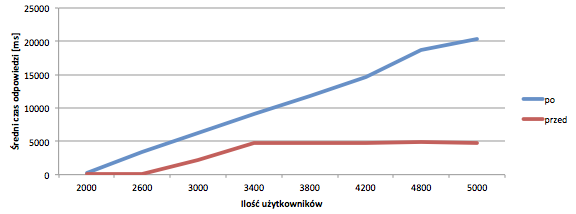
\includegraphics[width=1\linewidth]{assets/sredni3.png}
		\caption{Przebieg średniego czasu odpowiedzi dla zakresu użytkowników od 2000 do 5000 po rekonfiguracji serwera}
	\label{fig:sred3}
\end{figure}

\begin{figure}[ht]
	\centering
		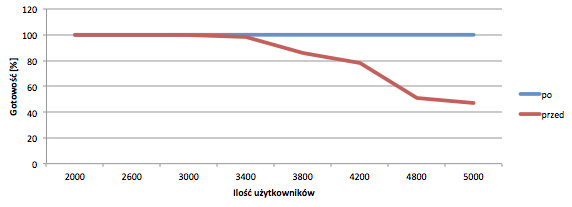
\includegraphics[width=1\linewidth]{assets/gotowosc3.png}
		\caption{Przebieg gotowości systemu dla zakresu użytkowników od 2000 do 5000 po rekonfiguracji serwera}
	\label{fig:got3}
\end{figure}
